\documentclass{article}
\usepackage[utf8]{inputenc}
\usepackage[russian]{babel}
\usepackage[left=2cm,right=2cm,
top=2cm,bottom=2cm,bindingoffset=0cm]{geometry}
\usepackage{graphicx}
\usepackage{amsmath}
\usepackage{float}
\usepackage{listings}
\usepackage{url,textcomp}
\date{2019 г.}
\author{Кондратенко Федор, гр 13632/1}
\setlength{\parindent}{0pt}
\setlength{\parskip}{5pt plus 2pt minus 1pt}
\frenchspacing
\title{Отчет по заданию №3.2}
\begin{document}
	\maketitle
	\section*{Модель}
	В качестве исходной была взята модель из задания 3.1. В нее был внесен ряд изменений, а именно:
	\begin{enumerate}
		\item Вместо коэффициента $b$ задается коэффициент $\psi$;
		\item Проведен рефакторинг системы, создана вспомогательная подсистема подсистемы для расчета коэффициентов;
		\item Добавлены блоки анализа системы.
	\end{enumerate}
	Внешний вид модели:
	\begin{figure}[H]
		\centering
		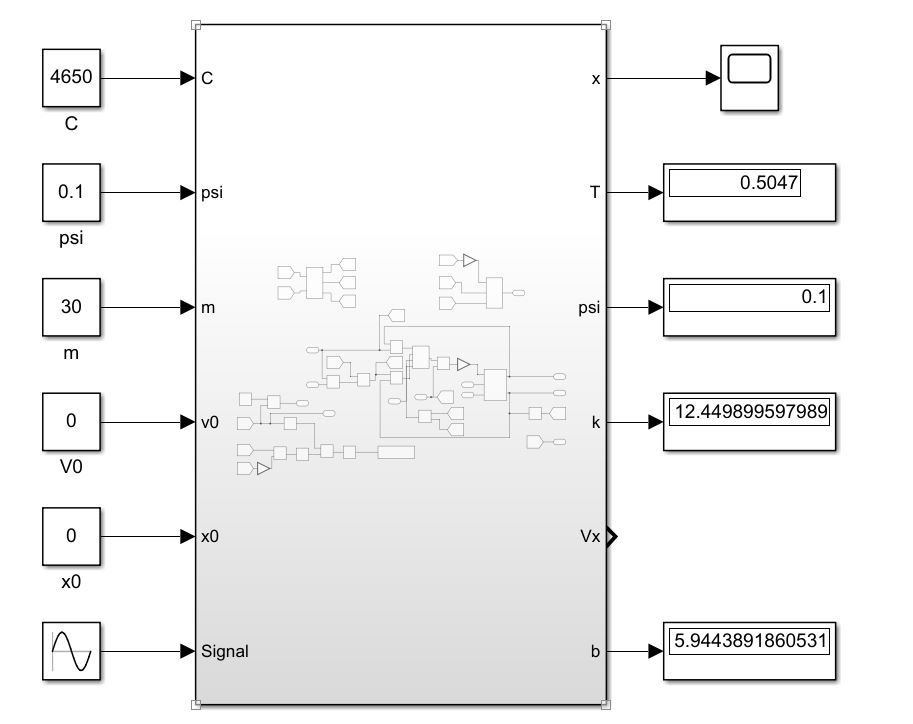
\includegraphics[width=0.7\linewidth]{model_outdoor}
		\caption{Внешний вид модели}
		\label{fig:modeloutdoor}
	\end{figure}
	Подсисистема:
	\begin{figure}[H]
		\centering
		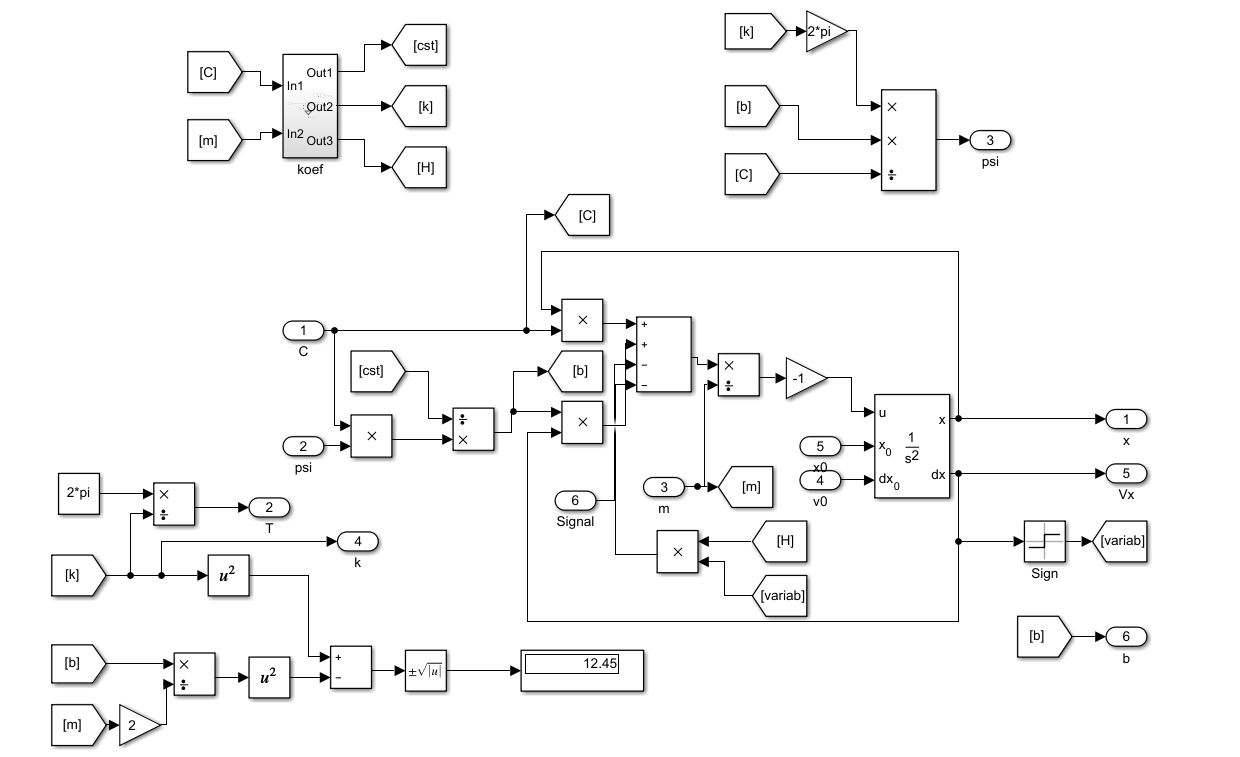
\includegraphics[width=1.1\linewidth]{model_all}
		\caption{Вид подсистемы}
		\label{fig:modelall}
	\end{figure}
	Дифференциальные уравнения колебаний остались теми же, за исключением уравнения для последнего задания.
	Вспомогательная подсистема:
	\begin{figure}[H]
		\centering
		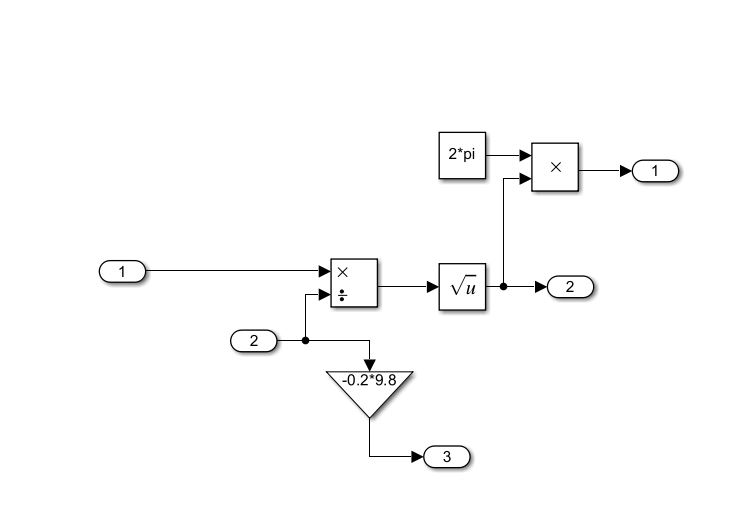
\includegraphics[width=0.7\linewidth]{koef}
		\caption{Вспомогательная подсистема. Вычисляет некоторые коэффициенты, которые далее используются при моделировании.}
		\label{fig:koef}
	\end{figure}
	\section*{Результаты моделирования и анализ системы}
	\begin{figure}[H]
		\centering
		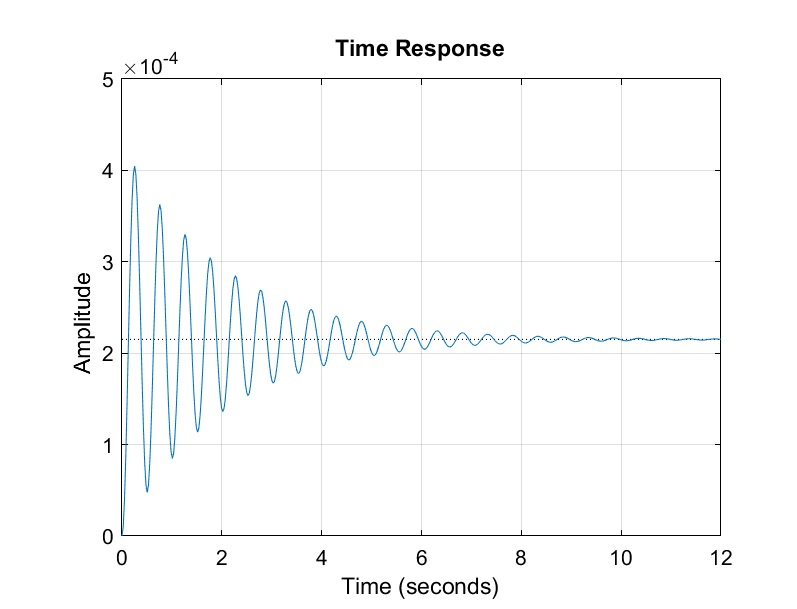
\includegraphics[width=0.7\linewidth]{graph2}
		\caption{Linear step response plot, $\psi = 0.5$}
		\label{fig:graph1}
	\end{figure}
	Время затухания свободных колебаний -- 8 секунд.
	\begin{figure}[H]
		\centering
		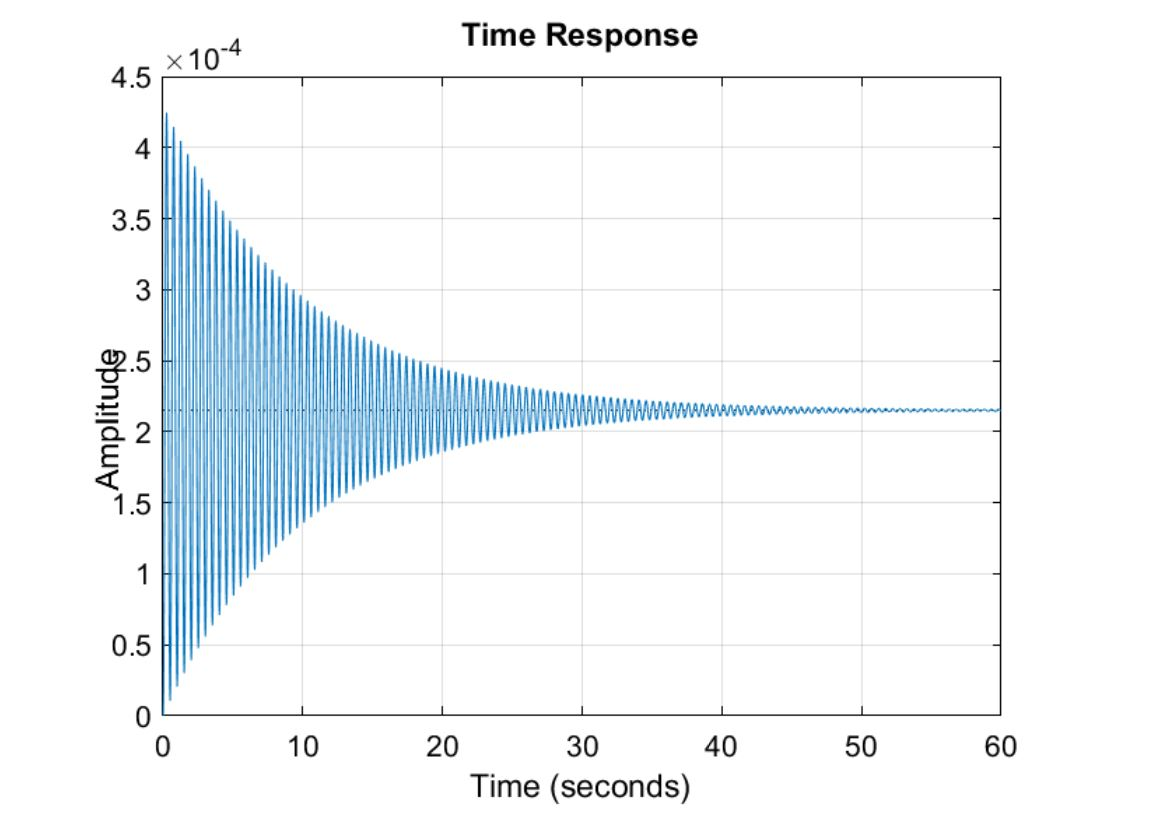
\includegraphics[width=0.7\linewidth]{graph1}
		\caption{Linear step response plot, $\psi = 0.1$}
		\label{fig:graph1}
	\end{figure}
	Время затухания свободных колебаний -- 40 секунд.
	Таким образом, уменьшение $\psi$ ведет к увеличению времени затухания свободных колебаний.
	\begin{figure}[H]
		\centering
		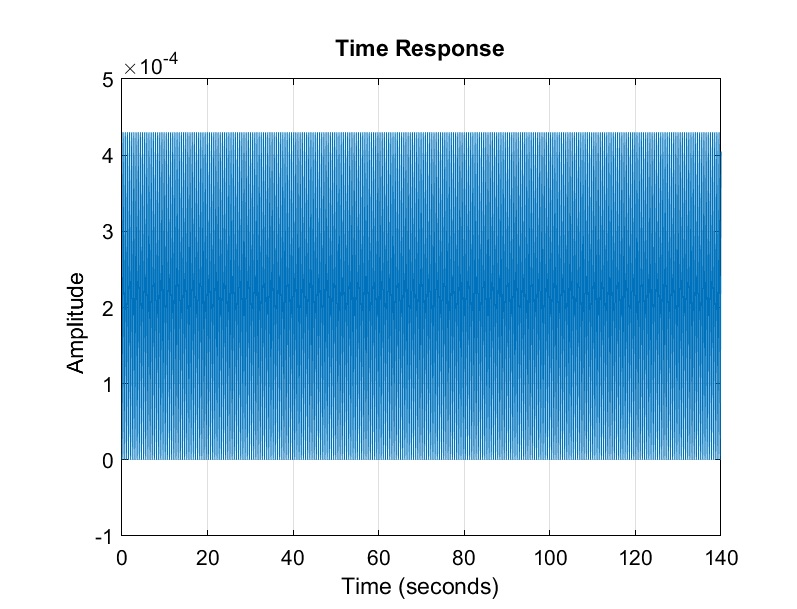
\includegraphics[width=0.7\linewidth]{graph3}
		\caption{Linear step response plot, $\psi = 0$}
		\label{fig:graph3}
	\end{figure}
	Время затухания свободных колебаний -- 40 секунд.
	Таким образом, уменьшение $\psi$ ведет к увеличению времени затухания свободных колебаний. При $\psi = 0$ колебания не затухают.
	\begin{figure}[H]
		\centering
		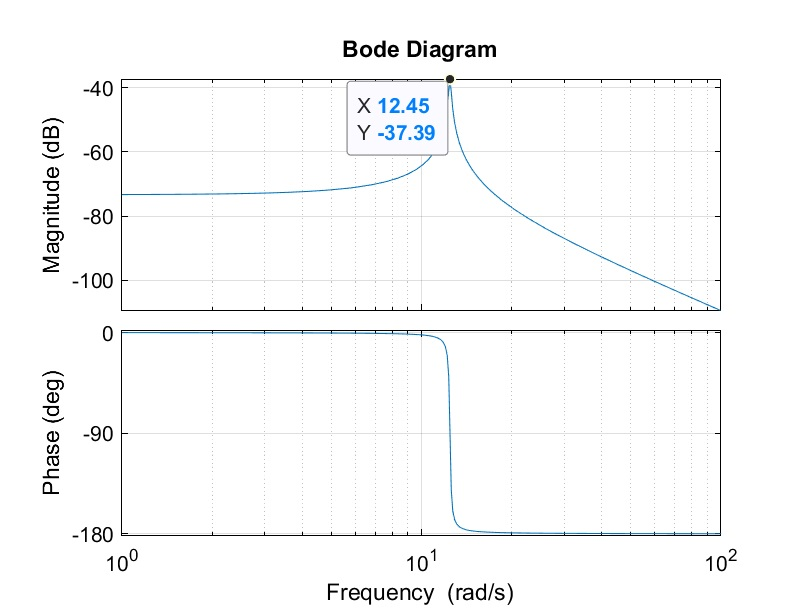
\includegraphics[width=0.7\linewidth]{graph4}
		\caption{АЧХ и ФЧХ системы, $\psi = 0.5$}
		\label{fig:graph4}
	\end{figure}
	\begin{figure}[H]
		\centering
		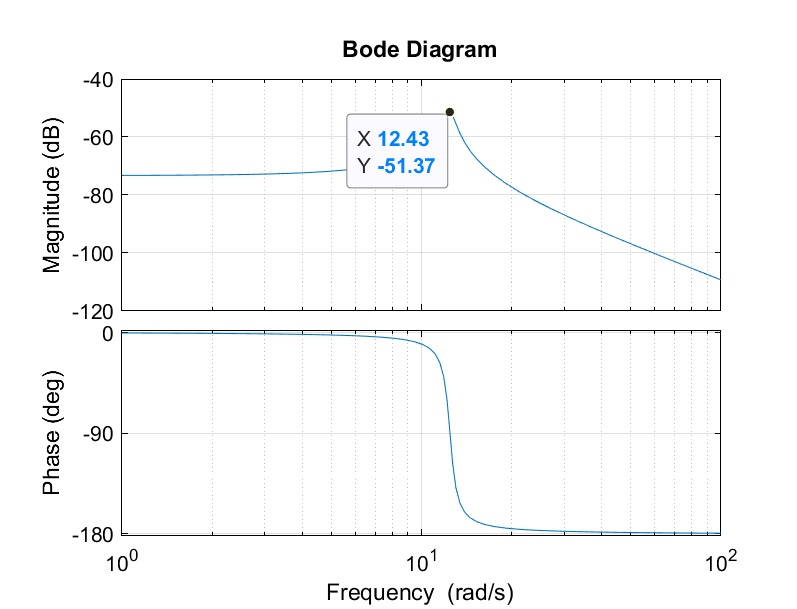
\includegraphics[width=0.7\linewidth]{graph5}
		\caption{АЧХ и ФЧХ системы, $\psi = 0.1$}
		\label{fig:graph5}
	\end{figure}
	\begin{figure}
		\centering
		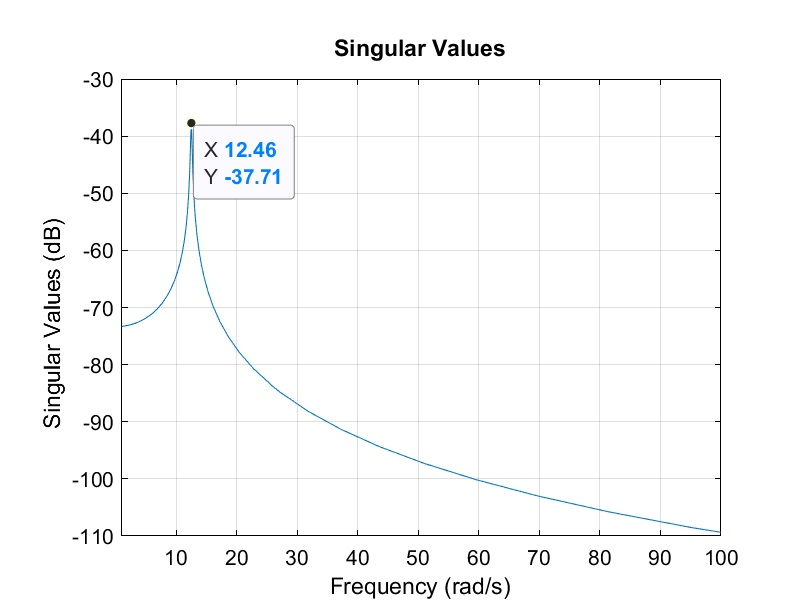
\includegraphics[width=0.7\linewidth]{graph6}
		\caption{Вид АЧХ при линейной шкале частот, $\psi = 0.5$}
		\label{fig:graph6}
	\end{figure}
	Как видно, при меньшем $\psi$ амплитуда на АЧХ становится больше, ФЧХ не меняется.
	\begin{figure}[H]
		\centering
		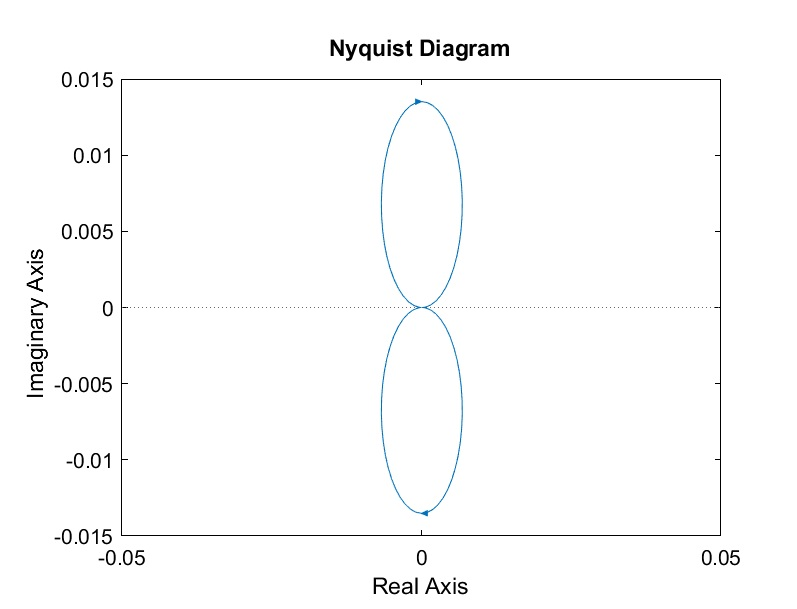
\includegraphics[width=0.7\linewidth]{graph7}
		\caption{АФЧХ системы, система усточива}
		\label{fig:graph7}
	\end{figure}
	\begin{figure}[H]
		\centering
		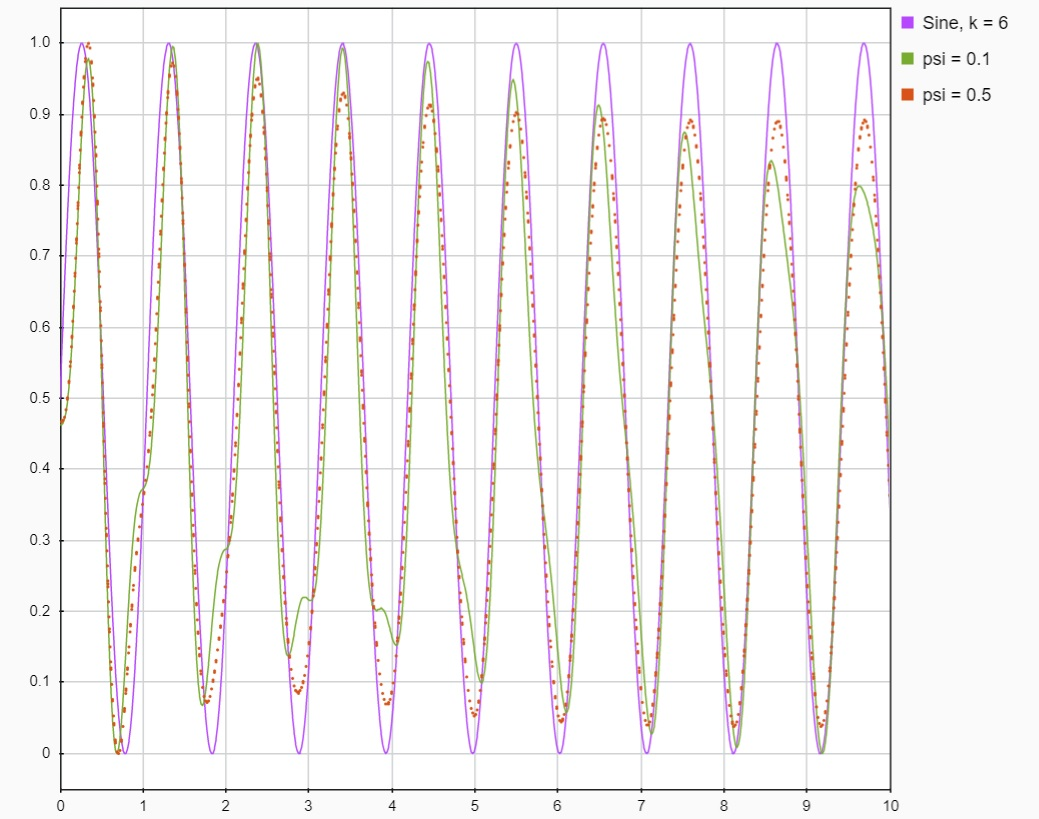
\includegraphics[width=0.7\linewidth]{signal1}
		\caption{Вынужденные колебания до резонанса, k = 6, колебания происходят в одной фазе}
		\label{fig:signal1}
	\end{figure}
	\begin{figure}[H]
		\centering
		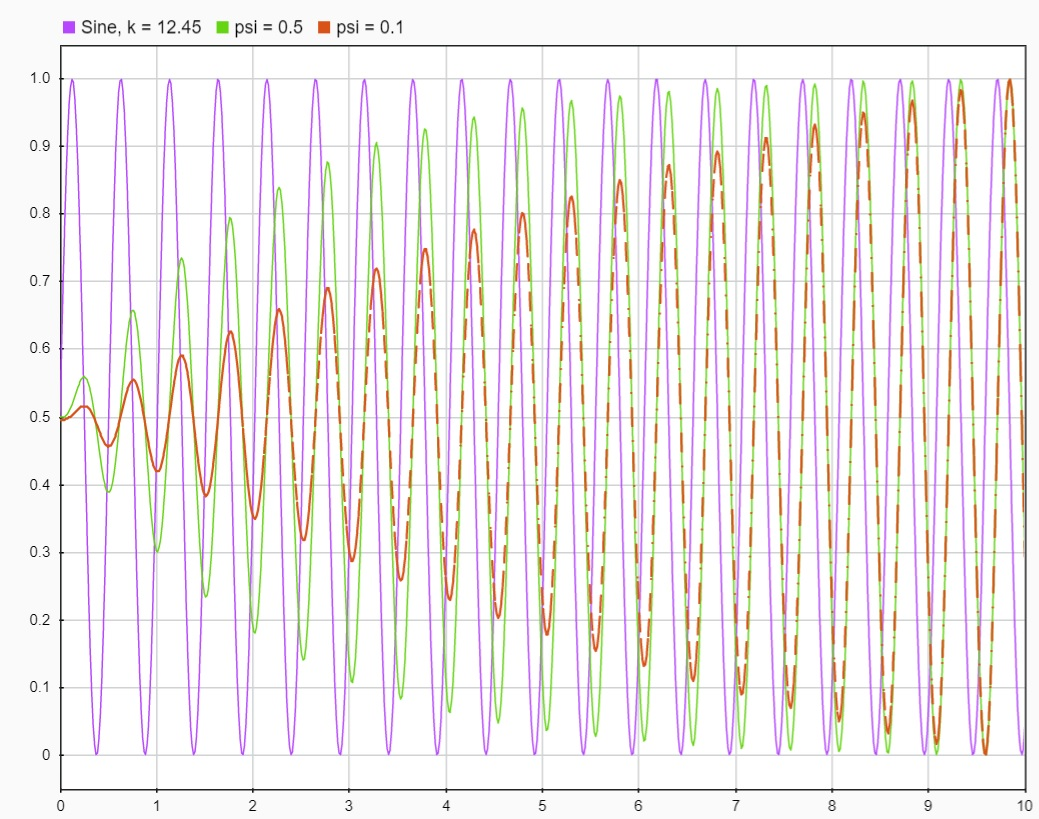
\includegraphics[width=0.7\linewidth]{signal2}
		\caption{Колебания на частоте резонанса, k = 12.45, сдвиг по фазе на $\frac{\pi}{2}$}
		\label{fig:signal2}
	\end{figure}
	\begin{figure}
		\centering
		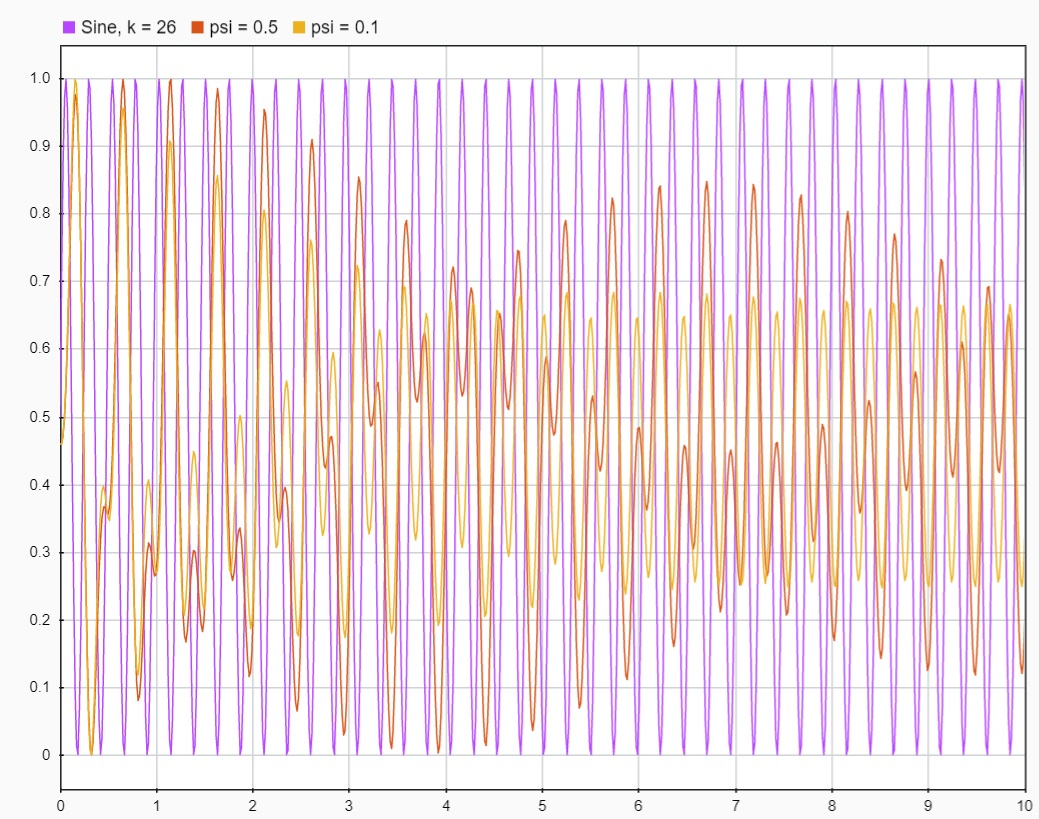
\includegraphics[width=0.7\linewidth]{signal3}
		\caption{Колебания после резонанса, k = 26, колебания происходят в противофазе с вынуждающей силой}
		\label{fig:signal3}
	\end{figure}
	
	\section*{Добавление в систему сухого трения}
	В связи с добавлением в систему сухого трения, дифференциальное уравнение колебаний меняется:
	$$mx''+bx'+cx=F_0sin(\omega t)-0.2*mg*sign(x')$$
	\begin{figure}[H]
		\centering
		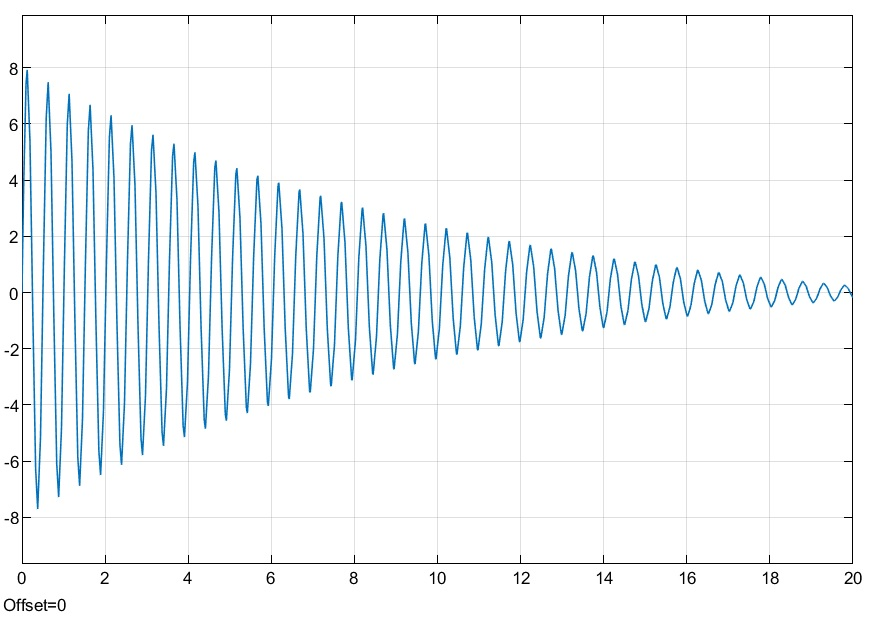
\includegraphics[width=0.7\linewidth]{suhtr1}
		\caption{Затухающие колебания при учете сухого трения}
		\label{fig:suhtr1}
	\end{figure}
	\begin{figure}[H]
		\centering
		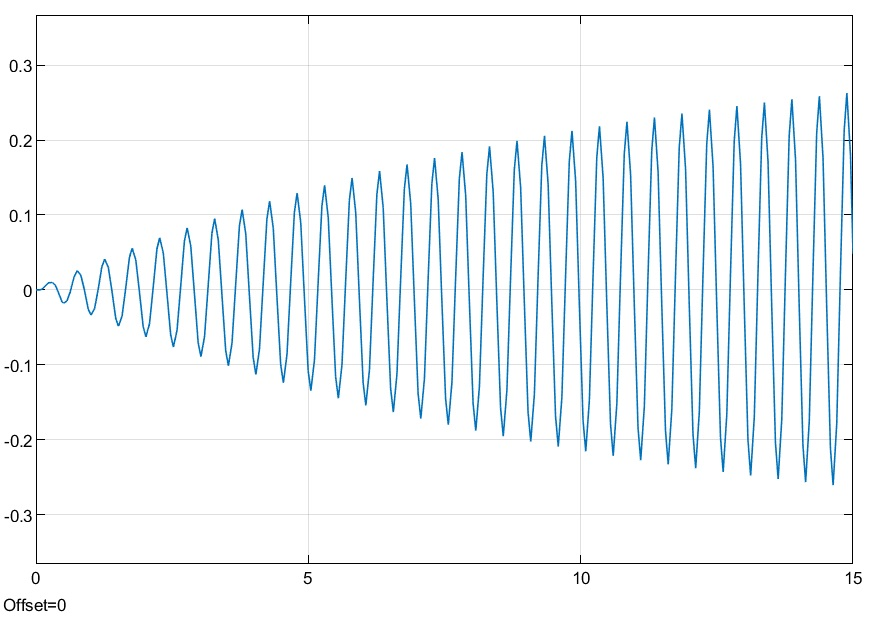
\includegraphics[width=0.7\linewidth]{suhtrres}
		\caption{Резонанс при учете сухого трения}
		\label{fig:suhtrres}
	\end{figure}
	"Экспоненциальность" амплитуды колебаний уменьшилась.
\end{document}